\chapter{Reti mobili e wireless}
\section{Introduzione}
In  una rete wireless si possono identificare:
\begin{itemize}
\item Host wireless: sono i dispositivi end system che eseguono applicazioni.
\item Link wireless: un host si connette ad una base station attraverso un wireless communication link.
\item Base station: \`e la componente fondamentale per inviare e ricevere dati da e per un host wireless che \`e associato con essa. \`E responsabile per la coordinazione della trasmissione di host multipli con la
quale \`e associata. L'associazione avviene quando l'host \`e a distanza comunicativa dalla base station e la utilizza per trasferire data tra essa e la rete. Host associati con una base station si definiscono come 
operanti in infrastructure mode.  
\item Network infrastructure: la rete con la quale un host vuole comunicare.
\end{itemize}
Queste componenti possono essere combinate in maniera diversa.
\begin{itemize}
\item Single-hop infrastructure-based: queste reti hanno una base station che \`e connessa ad una rete cablata e la comunicazione tra questa base station e l'host wireless avviene lungo un singolo wireless hop.
\item Single-hop infrastructure-less: non esiste una base station ma uno dei nodi pu\`o svolgere il ruolo di coordinare la trasmissione degli altri.
\item Multi-hop, infrastructure-based: \`e presente una base station che \`e cablata alla rete ma alcuni nodi wirless potrebbero dover relay la loro comunicazione attraverso altri nodi wireless in modo da 
comunicare con la base station.
\item Multi-hop, infrastructure-less: non c'\`e una base station  e i nodi potrebbero dover relay messaggi attraverso moli altri nodi per raggiungere la destinazione. 
\end{itemize}
\section{Link wireless e caratteristiche della rete}
Le maggiori differenze tra una rete cablata e wireless sono:
\begin{itemize}
\item Decreasing signal strength: radiazioni elettromagnetiche si attenuano mentre passano attraverso la materia causando attenuazione del segnale mentre i due dispositivi si allontanano.
\item Interference da altre sorgenti: sorgenti che trasmettono alla stessa frequenza interferiscono tra di loro. 
\item Multipath propagation: questo fenomeno accade quando porzioni dell'onda elettromagnetica vengono riflesse prendendo cammini di lunghezza diversa tra un mittente ed un destinatario.
\end{itemize}
Gli errori bit accadono molto frequentemente, vengono pertanto impiegati codici di individuazione errori CRC potenti e protocolli di data transfer affidabili a livello di link. L'host riceve un segnale 
elettromagnetico che \`e una combinazione di una forma degradata del segnale trasmesso. Il signal-to-noise ration (SNR) \`e una misura relativa della forza del segnale ricevuto e il rumore. \`E misurata 
tipicamente in decibel maggiore \`e questo valore pi\`u \`e facile per il ricevente estrarre il segnale trasmesso dal rumore di fondo. Si dice la probabilit\`a che un bit trasmesso sia ricevuto in errore al ricevente
come bit error rate.
\begin{itemize}
\item Per uno schema di modulazione pi\`u \`e alto l'SNR pi\`u basso il BER essendo che un mittente pu\`o aumentare l'SNR aumentando il potere di trasmissione si pu\`o pertanto diminuire il BER. 
\item Per un dato SNR una tecnica di modulazione con un tasso di trasmissione maggiore pi\`u alto avr\`a un maggiore BER. 
\item Selezione dinamica della tecnica di modulazione del livello fisico pu\`o essere utilizzata per adattare la tecnica di modulazione alle condizioni del canale. 
\end{itemize}
Nel caso di un link wireless pu\`o essere difficile fare broadcast a causa di interferenza e collisioni invisibili causate dal fading della forza di un segnale. 
\subsection{CDMA}
Quando un host comunica su un mezzo condiviso \`e necessario un protocollo \`e necessario in modo che i segnali inviati da mittenti multipli non interferiscano al ricevente. CDMA appartiene alla famiglia dei
protocolli di channel partitioning \`e prevalente nelle LAN wireless. In un protocollo CDMA ogni bit inviato \`e codificato moltiplicando il bit da un segnale che che cambia ad un tasso maggiore della sequenza 
originale. Si supponga che il tasso in cui bit di dati entrano nel codificatore CDMA definiscano l'unit\`a di tempo, nel senso che ogni bit da essere trasmesso richiede un one bit slot time. Sia $d_i$ il valore del
data dit all'iesimo bit slot. Ogni bit slot \`e sottodiviso in $M$ mini-slots. Il codice CDMA utilizzato dal mittente consiste di una sequenza di $M$ valori $c_m$ ognuno dei quali prende valore $1$ o $-1$. Per
ogni m-esimo mini slot del tempo di trasmissione di $d_i$ l'output del codificatore CDMA $>_{i,m}$ \`e il valore di $d_i$ moltiplicato dall'm-esimo bit del codice CDMA. Se non ci fossero mittenti che
interferiscono i dati originali sono ricomposti computando $d_i=1M\sum m 01MZ_imc_m$. Per recuperare i dati in presenza di interferenza si assume che i segnali di interferenza sono additivi. Nella presenza 
di mittenti multipli il mittente $s$ computa la trasmissione e il valore ricevuto al ricevente all'm-esimo mini slot dell'i-esimo bit slot \`e la somma dei bit trasmessi da tutti gli $N$ invianti durante quel mini slot.
Se i codici dei mittenti ogni ricevente pu\`o recuperare i dati inviati da un dato mittente dal segnale aggregato utilizzando il codice del mittente nella stessa maniera utilizzata per codificarlo. 
\section{LANs wireless 802.11: WiFi}
La tecnologia prevalente per le LAN wireless \`e la IEEE 802.11 wireless LAN o WiFi. Il protocollo di accesso \`e CSMA/CA. Ha l'abilit\`a di ridurre il tasso di trasmissione in modo da raggiungere distanza 
maggiori. Sono anche compatibili con le fersioni precedenti. Le versioni sono diverse sul livello fisico. 
\subsection{L'architettura 802.11}
Le componenti fondamentali dell'architettura 802.11 sono il basic service set (BSS) che contiene delle stazioni wireless e una base station centrale conosciuta come access point (AP) e un router che connette la
BSS all'internet. Come i servizi ethernet ogni stazione wireless ha un indirizzo MAC a 6 byte slavata nel firmware del suo adattatore e ogni AP ne ha uno per la sua interfaccia wireless. Sono chiamate 
infrastracture wireless LANs con l'infrastruttura il AP con la connessione ethernet che la connette al router. 
\subsubsection{Canali e associazione}
In 802.11 ogni stazione wireless deve associarsi con un AP prima che possa inviare o ricevere datagrammi. Quando un amministratore di rete installa un AP assigna un Service Set Identifier (SSID) all'access 
point e un numero di canale. Questo standard opera nel range di frequenza 2.4 GHz e 2.4835 GHz. Attraverso questa banda di 85 MHz vengono definiti 11 canali parialmente sovrapposti. Si indica con
WiFi jungle una locazione fisica dove una stazione riceve segnale forte da due o pi\`u APs vicine. Per accedere all'Internet il dispositivo deve entrare una delle sottoreti e associarsi con una delle APs. Associarsi
vuol dire che il dispositivo crea un cavo virtuale tra s\`e stesso e l'AP. Solo l'AP invier\`a data frames al dispositivo wireless e viceversa. Lo standard richiede che un AP invii periodicamente beacon frames ognuno 
di quali include l'SSID dell'AP e l'indirizzo MAC. Il dispositivo wireless scansiona gli 11 canali cercando beacon frames da qualsiasi AP che ci potrebbe essere. Una volta appresi gli AP disponibili il dispositivo ne
seleziona uno per l'associazione. Tipicamente il dispositivo sceglie l'AP il cui beacon frame \`e ricevuto con la potenza massima del segnale. Il processo della scansione dei canali e l'ascolto per beacon frames \`e
conosciuta come passive scanning. Un dispositivo wireless pu\`o anche svolgere active scanning broadcasting un probe frame che sar\`a ricevuto da tutte le AP nel raggio. Un AP risponde al probe request frame
con un probe request frame. Il dispositivo wireless pu\`o scegliere l'AP con la quale associarsi tra quelle rispondenti. Dopo aver selezionato un AP con cui associarsi il dispositivo wireless invia un association 
request frame all'AP e l'AP risponde con un association response frame. Questo secondo handshak e\`e necessario in active scanning. Una volta associato il dispositivo vorr\`a unirsi alla sottorete e invier\`a
un DHCP discovery message nella sottorete attraverso l'AP in modo da ottenere un indirizzo IP. In modo per creare un associazione il dispositivo potrebbe dover autentificarsi con l'AP. Un approccio tra quelli
messi a disposizione con lo standard \`e quello di permettere accesso basata sull'indirizzo MAC. Un secondo approccio utilizza username e passwords. In entrambi i casi AP comunica con un server di 
autentificazione trasportando informazioni tra i dispositivi wireless e il server di autentificazione utilizzando un protocollo come RADIUS o DIAMETER.
\subsection{Il protocollo MAC 802.11}
Una volta che un dispositivo wireless \`e associato con un AP pu\`o cominciare a inviare e ricevere data frames con l'accesso point. Essendoci pi\`u dispositivi connessi si rende necessario un protocollo di 
multiple access per coordinare le trasmissioni. Viene utilizzato un random access protocol: il CSMA con collision avoidance (CSMA/CA). Ogni stazione sense il canale prima di trasmettere e si ferma dal 
trasmettere quando il canale \`e sensed impegnato. Utilizza tecniche di collision-avoidance e a causa dell'alto tasso di errore utilizza un metodo link-layer di acknowledgement/retransmission (ARQ) scheme.
Il protocollo MAC on implementa collision avoidance in quanto l'abilit\`a di individuare collisione richiede l'abilit\`a di inviare e ricevere allo stesso tempo e anche se ne fosse capace alcune collisioni non 
sarebbero identificati. Una volta che una stazione inizia a trasmettere un frame lo trasmette interamente. Si consideri prima il link-layer acknowledgement- Quando una stazione destinataria riceve un frame che
passa il CRC aspetta un periodo conosciuto come Short inter-frame Spacing (SIFS) e poi  ritorna un frame di acknowledgement. Se la stazione non riceve un acknowledgement in un periodo dato assume che un
errore \`e accaduto e ritramsette il frame utilizzando il protocollo CSMA/CA per accedere al canale. Se un acknowledgement non \`e ricevuto dopo un numero di ritrasmissioni elimina il frame. Si supponga che
una stazione abbia un frame da inviare:
\begin{itemize}
\item Se la stazione sense il canale idle trasmette il frame dopo un intervallo di Distributed inter-frame Space (DIFS).
\item Altrimenti la stazione sceglie un valore di random backoff utilizzando binary exponential backoff e conta questo valore dopo DIFS quando il valore \`e sensed idle. Quando il canale \`e occupato il contatore
rimane fermo.
\item Quando il contatore arriva a zero la stazione trasmette l'intero frame e aspetta per un acknowledgement.
\item Se un acknowledgement \`e ricevuto la stazione sa che il frame \`e stato trasmesso correttamente, se ha un altro frame inizia il protocollo al punto due, se non \`e ricevuto rientra la fase di backoff con un
valore randomico scelto con un intervallo pi\`u larog.
\end{itemize}
\subsubsection{Gestire terminali nascosti: RTS e CTS}
Il protocollo 802.11 MAC include un meccanismo di reservation che aiuta evitare collisioni nella presenza di terminali nascosti. Si supponga che ci siano due stazioni wireless e un access point. Entrambe le
stazioni sono in range dell'AP e sono associate con essa ma le stazioni sono nascoste l'una dall'altra. In modo da evitare le collisioni si pu\`o utilizzare frame di controllo request to send (RTS) e clear to send 
(CTS) per riservare accesso al canale. Quando un mittente vuole inviare data frame pu\`o prima invare un RTS all'AP indicando il tempo totale richiesto per trasmettere essi e l'ACK. Quando un AP riceve un RTS
risponde broadcasting un CTS frame che d\`a al mittente permesso esplicito di inviare e istruisce le altre stazioni di non inviare per la durata riservata. Questo meccanismo migliora le prestazioni mitigando il 
problema delle stazioni nascoste e creando poche collisioni tra TRS e CTS, ma introduce ritardi e consuma risorse di canale, viene pertanto utilizzato solo per lunghi data frames. 
\subsection{Il frame IEEE 802.11}
Il frame IEEE 802.11 condivide molte similitudini con un frame ethernet contiene un numero di campi specifici per il suo utilizzo wireless.
\begin{figure}[h]
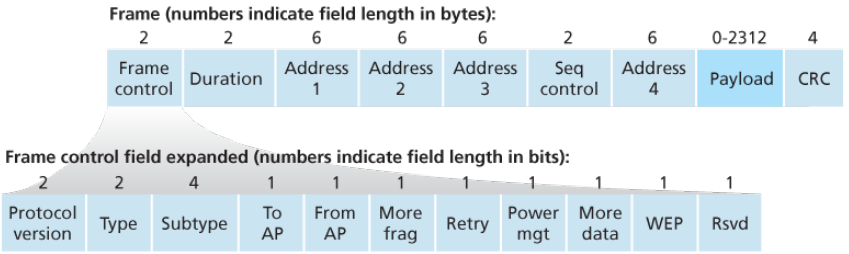
\includegraphics[width=\textwidth]{Frame80211.png}
\caption{Struttura di un frame 802.11}
\end{figure}
\subsubsection{Campi payload e CRC}
Tipicamente il payload consiste di un datagramma IP o di un pacchetto ARP, tipicamente limitato a 1500 bytes. Viene incluso un 32-bit cyclic redundancy check in modo da poter individuare errori. 
\subsubsection{Campi di indirizzo}
Il frame possiede quattro campi di indirizzo ognuno dei quali contiene un indirizzo MAC a 6 bytes. Tre campi sono necessari per scopi di internetworking: per muovere il datagframma dalla stazione all'AP al
router. Il quarto indirizzo \`e utilizzato quando un AP forward pacchetti in modalit\`a ad-hoc. 
\begin{itemize}
\item L'indirizzo 2 \`e l'indirizzo MAC della stazione che trasmette il frame. 
\item L'indirizzo 1 \`e l'indirizzo MAC della stazione wireless che deve ricevere il frame. 
\item L'indirizzo 3 contiene l'indirizzo MAC dell'interfaccia router della sottorete in cui si trova la stazione wireless, svolge un ruolo fondamentale di comunicazione tra la rete wireless e cablata.
\end{itemize}
\subsubsection{Sequence number, durata  e campi di frame control}
Il sequence number viene utilizzato per mappare l'acknowledgement al pacchetto su cui agisce. Il campo di durata include il periodo in cui una stazione riserva la connessione per inviare un frame e 
l'acknowledgement, incluso in RTS e CTS. Il campo frame control possiede molti sottocampi: il tipo e il sottotipo sono utilizzati per distinguere tra frame di associazione, di dati, RTS, CTS e ACK. I campi to e 
from definiscono i significati dei diversi campi di indirizzo. Il campo WEP indica se \`e utilizzata criptazione.
\subsection{Mobilit\`a nella stessa sottorete IP}
In modo da aumentare il raggio fisico di una LAN wireless vengono utilizzate multiple BSS con lo stessa sottorete IP. Si crea il problema di mantenere connesioni TCP spostandosi da una BSS all'altra. Quando
un dispositivo si sposta tra BSS mantiene l'indirizzo IP. Mentre il dispositivo si allontana individua un segnale che si indebolisce dall'Ap e comincia la scansione per un segnale pi\`u forte. Quando riceve un 
beacon frame si disassocia da quella corrente e si associa con l'altra mantenendo l'indirizzo IP e le connessioni TCP. Per aggiornare le tabelle di forwarding degli switch l'AP corrente invia un frame ethernet 
broadcast con l'indirizzo del dispositivo che si \`e appena connesso. 